\documentclass{article}
\usepackage[utf8]{inputenc}

\usepackage{sectsty}
\usepackage{fancyhdr}
\usepackage[top=1.25cm, bottom=2cm, left=2cm, right=2cm]{geometry}
\usepackage{tabularx,tabulary}
\usepackage{graphicx}
\date{Mardi 26 Mars 2019}
\author{KADOCH Daoud\\LEFEVRE Sebastien}
\title{\LARGE{Rapport 3I025\\}Cahier des Charges}
\usepackage[french]{babel}
%\usepackage[utf8x]{inputenc}
%\usepackage{amsmath}
%\usepackage[colorinlistoftodos]{todonotes}
\begin{document}

\begin{titlepage}

\newcommand{\HRule}{\rule{\linewidth}{0.5mm}} % Defines a new command for the horizontal lines, change thickness here

\center % Center everything on the page
 
%----------------------------------------------------------------------------------------
%	HEADING SECTIONS
%----------------------------------------------------------------------------------------

\textsc{\LARGE Université Pierre-et-Marie-Curie}\\[3cm] % Name of your university/college
\textsc{\Large Licence Informatique 3\up{ème} Année}\\[0.5cm] % Major heading such as course name
\textsc{\large 3I025}\\[2cm] % Minor heading such as course title

%----------------------------------------------------------------------------------------
%	TITLE SECTION
%----------------------------------------------------------------------------------------

\HRule \\[0.4cm]
{ \huge \bfseries Rapport 3I025}\\[0.4cm] % Title of your document
\HRule \\[2cm]
 
%----------------------------------------------------------------------------------------
%	AUTHOR SECTION
%----------------------------------------------------------------------------------------

\begin{minipage}{0.4\textwidth}
	\begin{flushleft} \large
	\emph{Auteurs:}\\[0.2cm]
	Daoud \textsc{KADOCH}\\ % Your name
	Sebastien \textsc{LEFEVRE} % Your name
	\end{flushleft}
\end{minipage}
~
\begin{minipage}{0.4\textwidth}
	\begin{flushright} \large
	\emph{Enseignant:} \\[0.2cm]
	Nicolas \textsc{MAUDET}
	\end{flushright}
\end{minipage}\\[4cm]

%----------------------------------------------------------------------------------------
%	DATE SECTION
%----------------------------------------------------------------------------------------

{\large Mardi 26 Mars 2019}\\[3cm] % Date, change the \today to a set date if you want to be precise

%----------------------------------------------------------------------------------------
%	LOGO SECTION
%----------------------------------------------------------------------------------------


\includegraphics[scale=0.15]{logo_sorbonne.PNG} % Include a department/university logo - this will require the graphicx package
 
%----------------------------------------------------------------------------------------

\vfill % Fill the rest of the page with whitespace

\end{titlepage}

% -----------------------------------------------------
\newpage
\renewcommand{\contentsname}{\center{Table des Matières}\vspace*{5cm}}

\tableofcontents

\newpage


\section{Contexte}
	Nous étudions un jeu multijoueur où plusieurs agents se voient attribuer une fiole et doivent simplement aller la chercher par le plus court chemin possible.\\
En plus d'éviter des obstacles, les joueurs ne doivent pas rentrer en collision entre eux. \\
Pour résoudre ce problème, nous allons étudier trois solutions distinctes en comparant leurs temps d'exécution afin de déterminer laquelle de ces trois approches est la meilleure.\\
On utilisera l'algorithme "A étoile", afin de calculer le plus court chemin d'un agent à une fiole.

\section{Stratégie Opportuniste}
	\subsection{Objectif}
		Cette solution consiste au tout début, à calculer un chemin avec
		l'algorithme "a étoile" pour chacun des joueurs, une fois ceci fait, le jeu peut démarrer et chaque joueur entame son propre parcours.\\ 
L'algorithme A étoile ne gérant pas les collisions entre les joueurs, nous allons donc imposer une loi qui indique que pour chacun des joueurs, avec c la case courante sur laquelle l'agent J se trouve, si un autre joueur J' se trouve à la case c+1, alors nous recalculons un chemin A étoile à partir de la case c pour J, en considérant J' comme un mur à ce même endroit.

	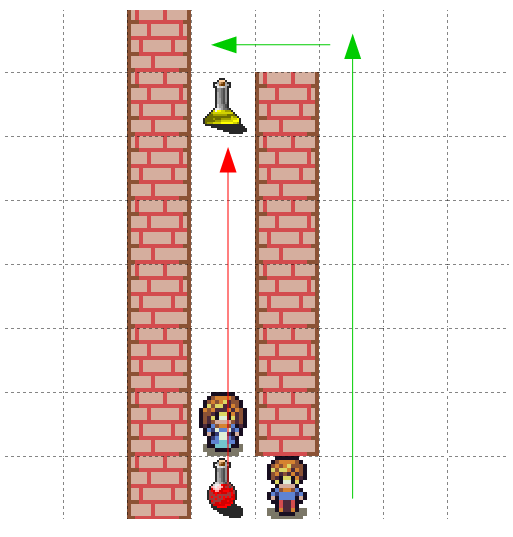
\includegraphics[scale=0.5]{Solution1_ex.png}

	Ce schéma illustre une situation dans laquelle le joueur J de case courante c (à droite de la fiole rouge) a pour chemin celui indiqué par la flèche rouge, et un autre joueur J'.\\
	Au prochain tour J' ira sur la case de la fiole rouge, pour empêcher une collision avec ce joueur, J va donc recalculer un nouveau chemin à l'aide de l'algorithme A étoile, qui est indiqué par les flèches vertes.

	\subsection{Résultats}
	
	Là on expose les résultats en fonction de quelques map.
	
	
\section{Stratégie Coopérative de Base}
	\subsection{Objectif}
	
	Dans cette solution, on calcule le chemin A étoile de chaque joueur dès le début à la manière de la stratégie opportuniste, néanmoins une étape préalable devra être exécutée.\\
	En effet pour la gestion des collisions nous allons étudier le chemin de chaque joueur et déterminer quels sont les joueurs qui peuvent exécuter leurs chemin en "parallèle" en formant des groupes de passage.\\
	Afin de former ces groupes, une méthode bien particulière est employée, en effet nous parcourons chaque chemins k des joueurs, et pour chaque case c de k, si c est présente dans un des chemins des autres joueurs, alors cela signifie que ces deux joueurs risquent une collision, ils ne passeront pas ensemble.\\
	A l'inverse si k n'a pas de case en commun avec un des joueurs, alors ils feront tous deux parti du même groupe de passage.
	Lorsque les groupes de passages sont établis, les groupes de joueurs peuvent donc passer les uns après les autres sans aucuns risque de collision.
	
	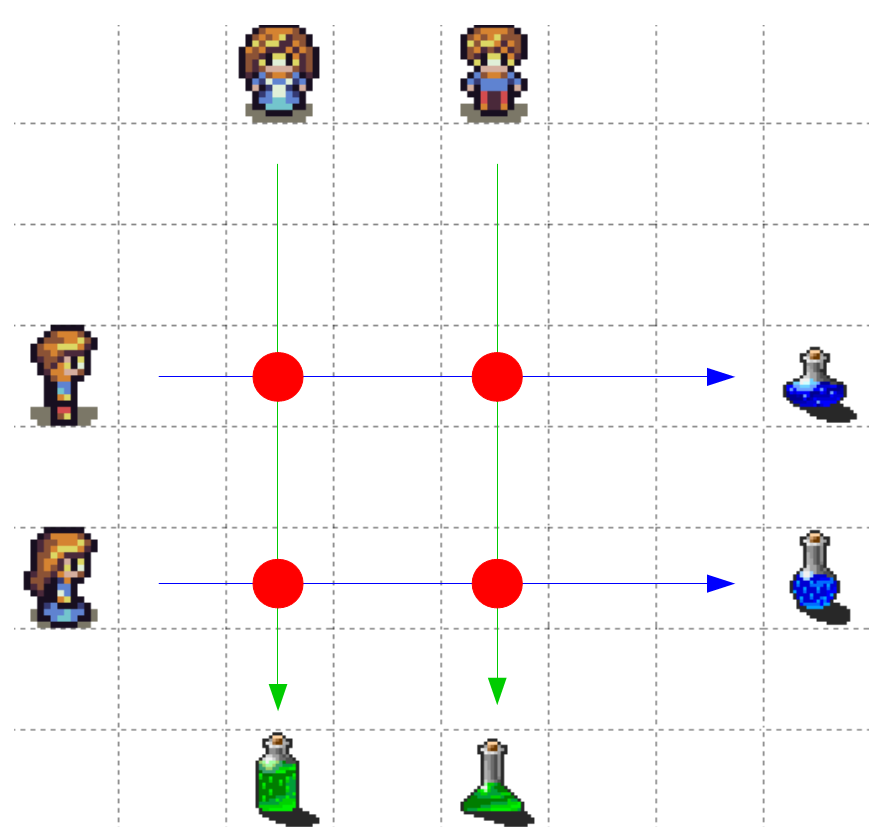
\includegraphics[scale=0.5]{Solution2_ex.png}
	
	Ce schéma illustre une situation avec quatre joueurs, nous observons ici quatre cases communes entre les joueurs qui ont été détectées par notre algorithme, représentées par les points rouges, les joueurs avec les chemins verts ne pourront pas passer avec les joueurs à chemin bleu et inversement car il y a un risque de collision.\\
	Nous pouvons donc distinguer ici deux groupes de passages : un premier groupe avec les chemins verts et un autre avec les chemins bleus.\\
	Si ces deux groupes passent l'un après l'autre, alors il n'y aura pas de risque de collision.\\


\end{document}